%! TEX root = ../thesis.tex
\section{Climpact}

\subsection{Web Platform}
\label{app:clm:climpact}

To collect data about people's perception from real users, we built the Climpact platform and opened it for students on our university campus.
Users answers questions in a quiz that asks them to compare pairs of actions.
They answer in relative terms, \textit{i.e.}, they indicate the relative order of magnitude between two actions, as shown in Figure~\ref{app:fig:climpactquiz}.
Once the quiz is finished, they have access to their answers that they can compare against the correct values (see Figure~\ref{app:fig:climpactanswers}.
Each action has its own page, and we display the perceived carbon footprint and the true values of several actions on one plot (see Figure~\ref{app:fig:climpactactions}.

\begin{figure}
	\centering
	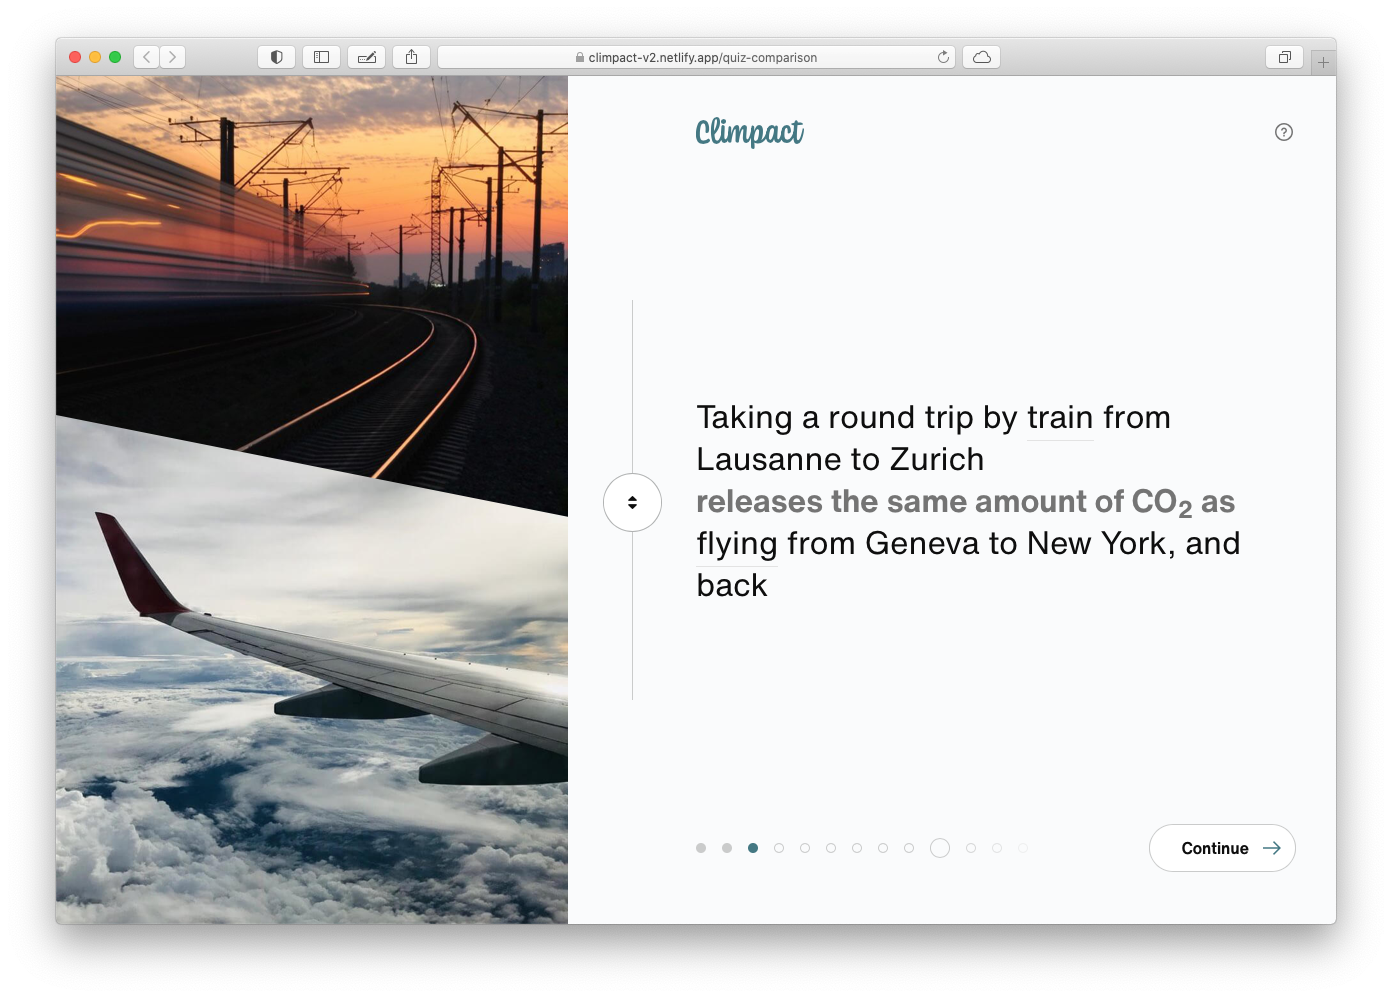
\includegraphics[width=0.96\textwidth]{climpact-quiz}
	\caption{Users answer simple questions in the form of pairwise comparisons.}
	\label{app:fig:climpactquiz}
\end{figure}

\begin{figure}
	\centering
	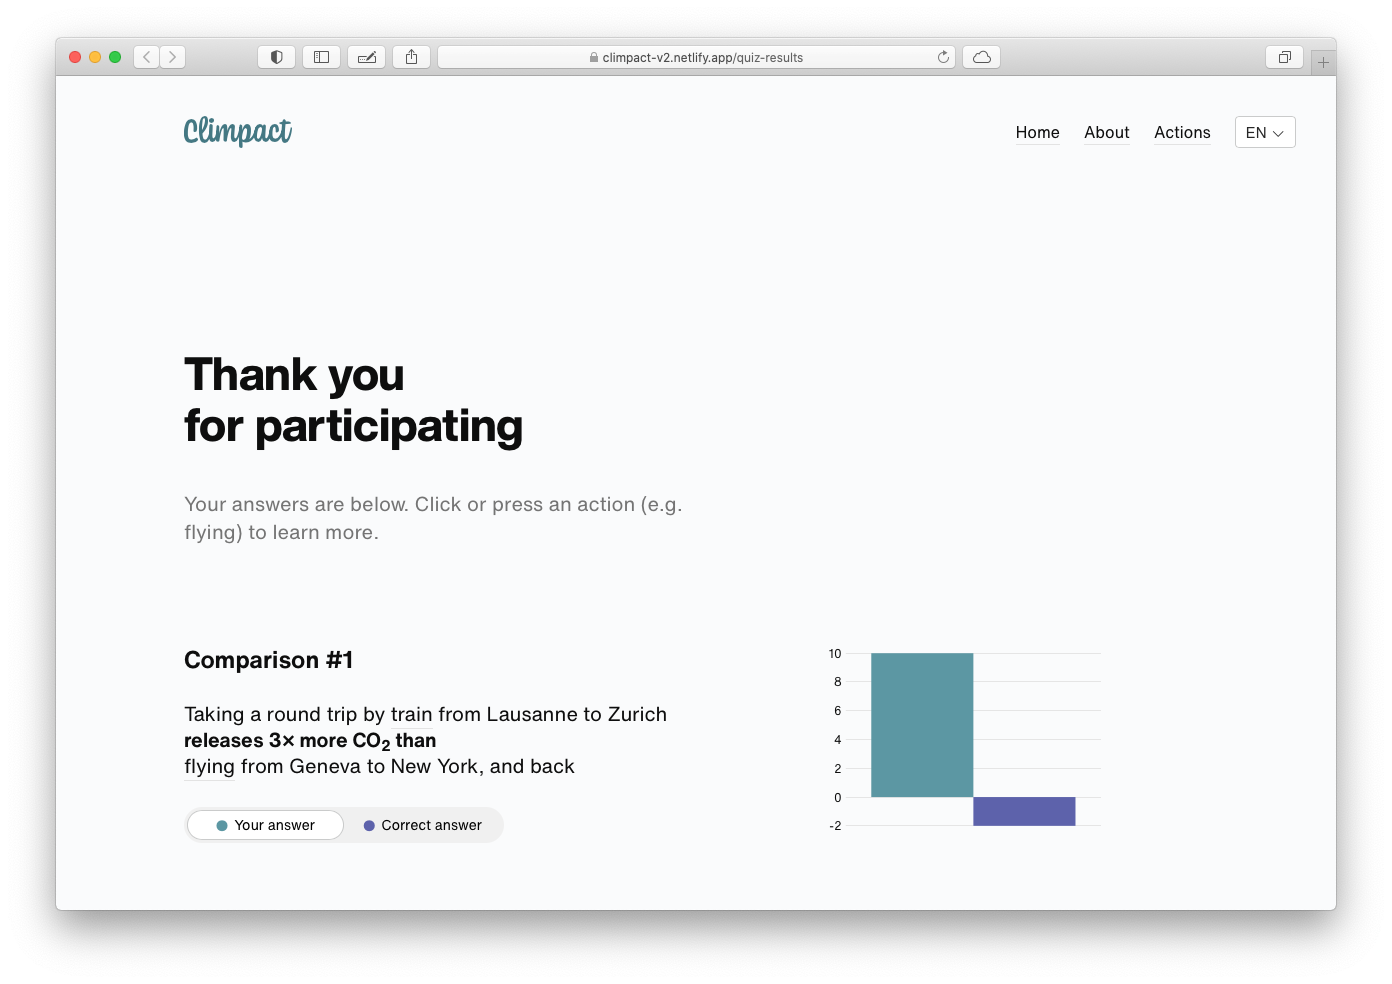
\includegraphics[width=0.96\textwidth]{climpact-answers}
	\caption{After the quiz, users can compare their answers with the correct ones.}
	\label{app:fig:climpactanswers}
\end{figure}

\begin{figure}
	\centering
	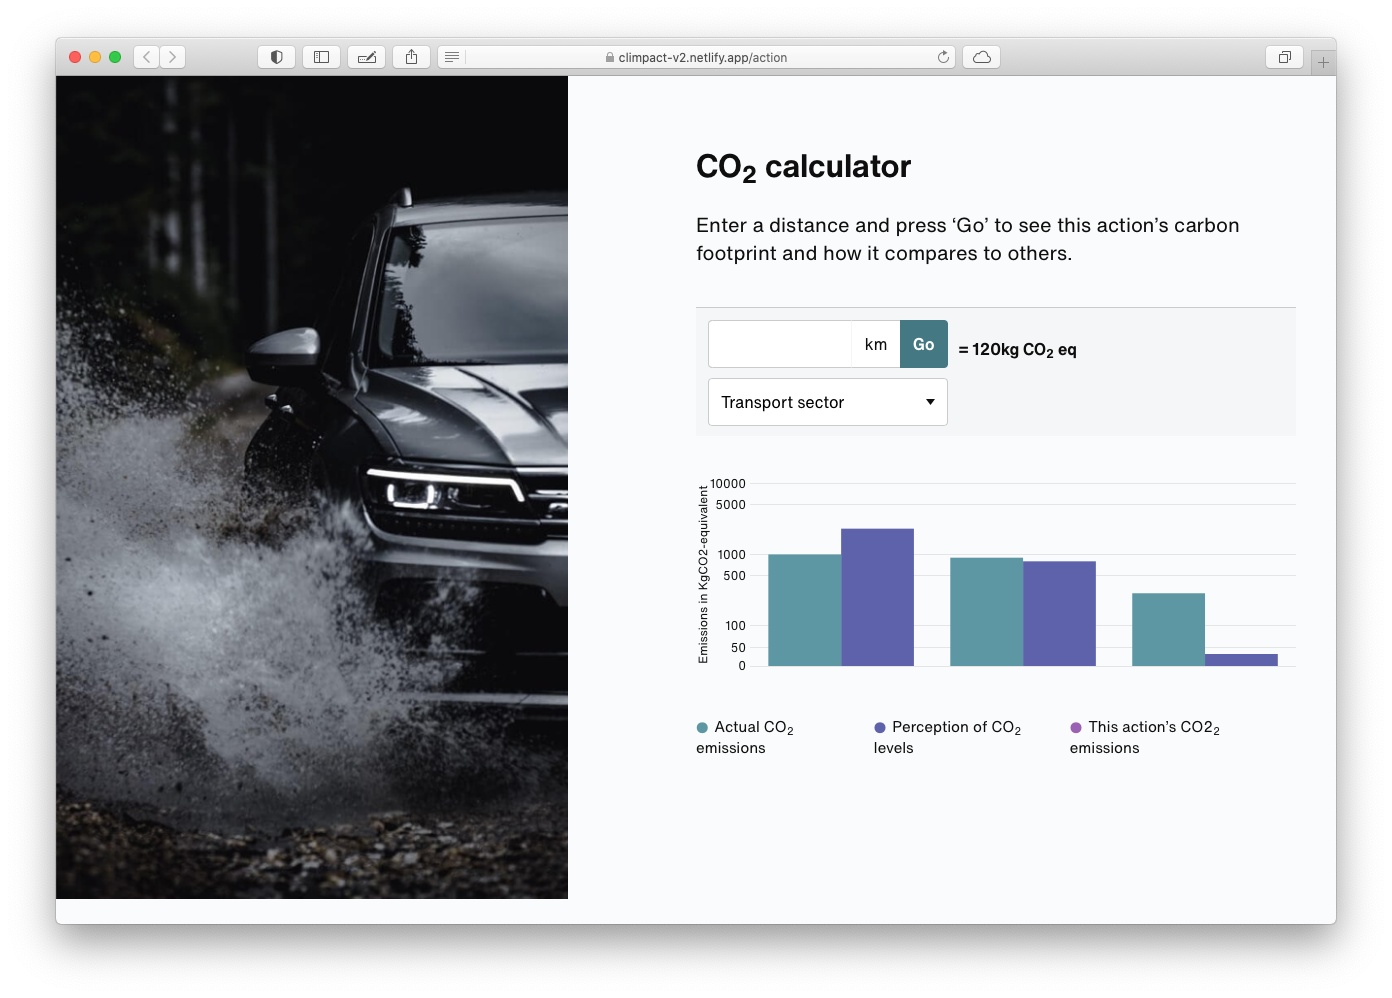
\includegraphics[width=0.96\textwidth]{climpact-actions}
	\caption{Each action has a page, where the perceive value for this action and the true values are displayed on a plot and compared with other actions.}
	\label{app:fig:climpactactions}
\end{figure}

\subsection{List of Actions}
\label{app:clm:actions}

We provide here the full list of actions, together with the true carbon footprint associated with each of them.
Because different countries use different sources of energy, we calculate the carbon footprint \textit{relative} to the country where our university is located.
The actions are ordered according to their true carbon footprint.
\begin{enumerateb}
	\item \actiontitle{Take the train in economy class on a 1000-km round-trip.} \\
	The train is a high-speed train with 360 seats.
	The seat-occupancy rate is 55\% (average rate for these types of trains).
	We count the \COtwo\ emissions per passenger. \\
	\actionvalue{17} % \cite{sncf2019calcul}
	\item \actiontitle{Dry your clothes with a dryer for one year.} \\
	A dryer emits \COtwo\ because it consumes electricity.
	We consider a dryer of average quality.
	The electricity is consumed from a grid with average \COtwo\ rate. \\
	\actionvalue{40} % \cite{wynes2017climate}
	\item \actiontitle{Light your house with LED bulbs.} \\
	LED bulbs emit CO2 because they consume electricity to generate light.
	The electricity is consumed from a grid with average \COtwo\ rate. \\
	\actionvalue{40} % [Appendix~\ref{app:bulbs}]
	\item \actiontitle{Take the bus on a 1000-km round-trip.} \\
	The bus is a standard-size bus with 60 seats.
	The seat-occupancy rate is 50\% (average rate for buses).
	We count the \COtwo\ emissions per passenger. \\
	\actionvalue{45} % \cite{mobitool,myclimate}
	\item \actiontitle{Drive an electric car alone on a 1000-km round-trip.} \\
	The car is a compact electric car that consumes 15 kWh/100km.
	The electricity is consumed from a grid with average \COtwo\ rate.
	There are no other passengers in the car.
	We count the \COtwo\ emissions per passenger. \\
	\actionvalue{45} % \cite{ofdl,myclimate,swissc02}
	\item \actiontitle{Car-share with three other persons on a 1000-km round-trip.} \\
	The car is a mid-sized gasoline car that consumes 7 l/100km.
	There are four persons in the car.
	We count the \COtwo\ emissions per passenger. \\
	\actionvalue{75} % \cite{ofdl,myclimate}
	\item \actiontitle{Eat local and seasonal fruits and vegetables for one year.} \\
	Growing food emits \COtwo\ because it requires fertilizing and driving agricultural machines.
	The goods are then transported to grocery shops and to your home. \\
	\actionvalue{89} % \cite{swissveg,foodmile}
	\item \actiontitle{Eat eggs and dairy products for one year.} \\
	The production of eggs and dairy products (milk, cheese, etc.) emits \COtwo\ because of water and land consumption, animal methane, and fossil fuel consumption for transportation and heating.
	We consider an average citizen consuming 50 kg of eggs and dairy products per year. \\
	\actionvalue{100} % \cite{wynes2017climate,viandesuisse}
	\item \actiontitle{Throw all waste in the same trash for one year.} \\
	Throwing all waste (PET, glass, cardboard, etc.) in the same trash, \textit{i.e.}, without recycling, emits \COtwo\ because more energy is needed to extract, transport, and process raw materials.
	Incinerators also burn more waste, and organic waste decomposition generates methane. \\
	\actionvalue{200} % \cite{wynes2017climate}
	\item \actiontitle{Light your house with incandescent bulbs.} \\
	Incandescent bulbs emit \COtwo\ because they consume electricity to generate light.
	The electricity is consumed from a grid with average \COtwo\ rate. \\
	\actionvalue{239} % [Appendix~\ref{app:bulbs}]
	\item \actiontitle{Fly in economy class for a 800-km round-trip.} \\
	The plane is a standard aircraft for short-distance flights with 180 seats.
	The seat-occupancy rate is 80\%.
	We count the \COtwo\ emissions per passenger. \\
	\actionvalue{270} % \cite{bofinger2013calculating,myclimate}
	\item \actiontitle{Drive alone for a 1000-km round-trip.} \\
	The car is a mid-sized gasoline car that consumes 7 l/100km.
	There are no other passengers in the car.
	We count the \COtwo\ emissions per passenger. \\
	\actionvalue{300} % \cite{mobitool,myclimate}
	\item \actiontitle{Heat your house with a heat pump for one year.} \\
	A heat pump emits \COtwo\ because it consumes electricity to generate heat.
	The house is of average size.
	The electricity is consumed from a grid with average \COtwo\ rate. \\
	\actionvalue{400} % \cite{energyenvironnement,swissenergyscope,swissc02}
	\item \actiontitle{Eat imported and out-of-season fruits and vegetables for one year.} \\
	Growing food emits \COtwo\  because it requires fertilizing and driving agricultural machines.
	Importing food emits \COtwo\ because of fossil fuel consumption for transportation.
	Out-of-season food emits \COtwo\ because it grows in greenhouse that needs to be heated.
	The goods are then transported to grocery shops and to your home. \\
	\actionvalue{449} % \cite{foodmile,swissveg}
	\item \actiontitle{Eat meat for one year.} \\
	Meat production emits \COtwo\ because of water and land consumption, animal methane, and fossil fuel consumption for transportation and heating.
	We consider an average citizen consuming 50 kg of meat per year. \\
	\actionvalue{800} % \cite{wynes2017climate,viandesuisse}
	\item \actiontitle{Fly in economy class for a 12000-km round-trip.} \\
	The plane is a standard aircraft for long-distance flights with 390 seats.
	The seat-occupancy rate is close to 100\%.
	We count the \COtwo\ emissions per passenger. \\
	\actionvalue{2300} % \cite{bofinger2013calculating,myclimate}
	\item \actiontitle{Heat your house with an oil furnace for one year.} \\
	An oil furnace emits \COtwo\ because it burns fuel to generate heat.
	The house is of average size. \\
	\actionvalue{3300} % \cite{energyenvironnement,swissenergyscope}
	\item \actiontitle{Fly in first class for a 12000-km round-trip.} \\
	The plane is a standard aircraft for long-distance flights with 390 seats.
	The seat-occupancy rate is close to 100\%.
	We count the \COtwo\ emissions per passenger.
	Passengers flying in first class use more space than passengers in economy. \\
	\actionvalue{9000} % \cite{bofinger2013calculating,myclimate}
\end{enumerateb}
